\section{Evaluation}
\label{sec:evaluation}

\subsection{Microbenchmarks}
\begin{figure*}[tb]
\centering
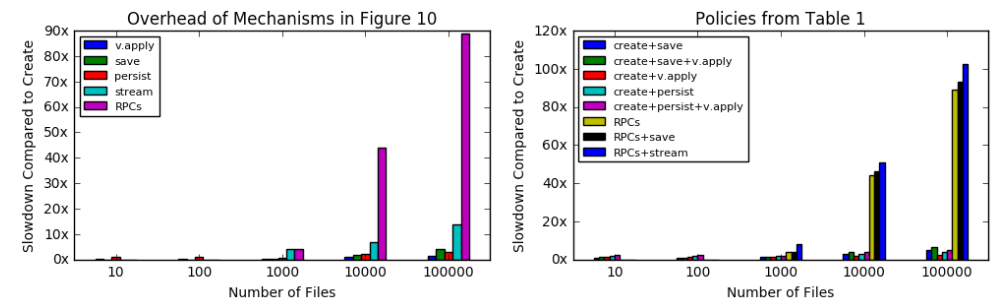
\includegraphics[width=180mm]{figures/results-microbenchmark.png}
\caption{Here's a graph.}
\end{figure*}

\begin{figure}[tb]
\centering
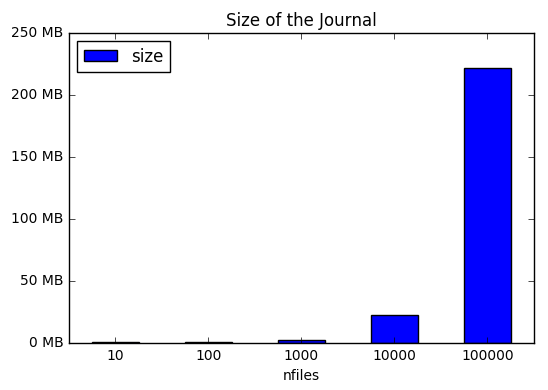
\includegraphics[width=90mm]{figures/results-files.png}
\caption{Here's a graph.}
\end{figure}


\subsubsection{Per phase latencies}
\begin{figure}[tb]
\centering
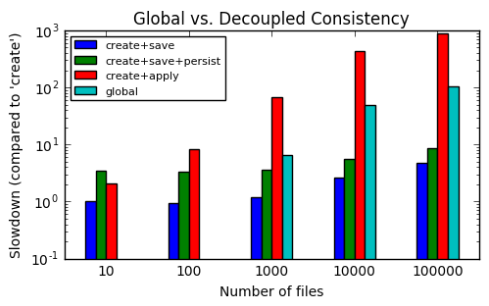
\includegraphics[width=90mm]{figures/global-v-decoupled.png}
\caption{Compared to the \texttt{create} phase, saving and persisting
updates (\texttt{create+save} and \texttt{create+save+persist}) experience only
a 4.79\(\times\) and 8.66\(\times\) slowdown, in the worst case for 100K files.
In contrast, maintaining \texttt{global} consistency is 905.70\(\times\)
slower.  The disadvantage of decoupling the namespace is the merge phase where
updates are applied to the metadata store (\texttt{create+apply}, resulting in a
905.70\(\times\) slowdown for 100K files.}\label{fig:global-v-decoupled}
\end{figure}

%\section{notes}
%Linking clients into our custom libcephfs
%
%Use namespace's recursive data structure to put policies on subtrees
%- consistency: eventual vs. strong, global vs. local
%  - e.g., BatchFS/DeltaFS: eventual, local
%  - e.g., POSIX: strong, global
%  - e.g., PLFS: no consistency
%- fault tolerance: global vs. local
%  - e.g., CephFS: global
%  - e.g., BatchFS/DeltaFS: local
%
%Experimental Setup
%- Ceph: 9 OSDs, 1 MDS, 2 kernel client
%- Workload limitations: blah
%
%Workload: creates
%
%Baseline: 200K creates in the same directory
%- throughput: degrades at 950s
%- CPU utilization: more at 950s
%- inode cache: eviction dominate
%- inodes +- to cache: eviction dominate
%- per-disk throughput: RADOS not bottleneck
%
%Experiment 1: Interference
%
%\subsection{Baseline}
%Experiment 0: creates in the same directory
%- setup: why we use caching, we use the kernel client, how we circumvent max fragment size
%
%Experiment 0: creates with a stat
%- Hypothesis: metadata read pauses creates and requires a snapshot in time
%  - what is more of an overhead: pausing creates and getting a consistent view OR sucking up resources as it reads from RADOS?
%- can we delay snapshot?
%
%Experiment 1: creates with a readdir
%- Hypothesis: shows the cost of synchronization because on a write, the first client drops his caps
%- client0: create 100k, client1: stat at 2 mins
%
%Experiment 2: scale the number of files
%- See if the open/close spike occurs 
%- Try to see why open/close spike is allowed to happen
%- Try to disable all caching -- metadata writes don't ever re-use the inode -- we never ask for it again!
%- client0: create 100k, client1: touch at 2 mins
%
%Experiment 3: see how fast the cache satisfies a read
%- client0: create 100k, stat inodes
%- client0: create 100k, client1: stat inodes
%
%lient 0: creates, client 1 create(s)

\subsection{Journaling Overhead}

Journal to RADOS
Turn off journaling (large segment)
Journal to in-memory OSD 

\subsection{Macrobenchmarks}
updatedb: http://lists.ceph.com/pipermail/ceph-users-ceph.com/2015-July/002768.html


